\documentclass{article}

\usepackage{tikz}
\usepackage{cancel}%for strikethrough
\usetikzlibrary{positioning}

\begin{document}


\begin{center}
\begin{minipage}{.2\textwidth}
\hspace*{-6cm}
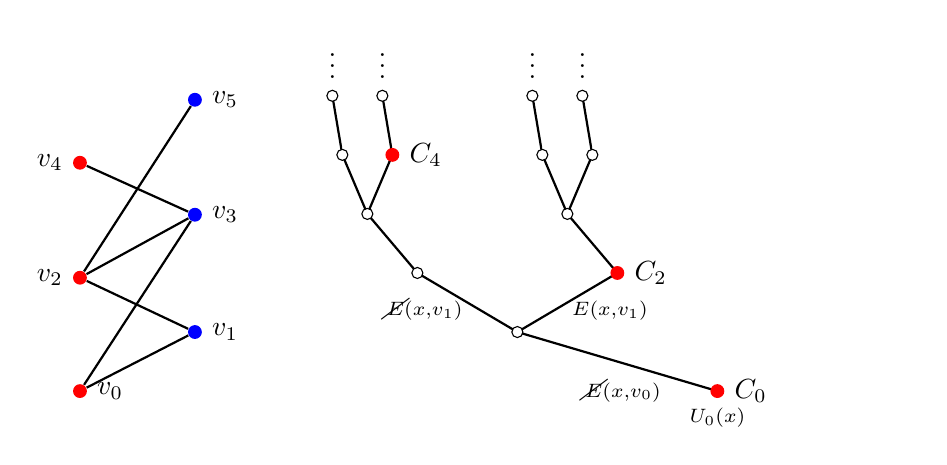
\begin{tikzpicture}[grow'=up,scale=.5]
\tikzstyle{level 1}=[sibling distance=4in]
\tikzstyle{level 2}=[sibling distance=2in]
\tikzstyle{level 3}=[sibling distance=1in]
\tikzstyle{level 4}=[sibling distance=0.5in]
\tikzstyle{level 5}=[sibling distance=0.2in]
\tikzstyle{level 6}=[sibling distance=0.1in]
\tikzstyle{level 7}=[sibling distance=0.07in]

\node {} coordinate (t9)
child{ coordinate (t0) edge from parent[color=black,thick]
child{coordinate (t00) edge from parent[color=black,thick]
child{coordinate (t000) edge from parent[color=black,thick]
child{coordinate (t0000) edge from parent[color=black,thick]
child{coordinate (t00000) edge from parent[color=black,thick]}
child{coordinate (t00001) edge from parent[color=white,thick]}
}%endparen for t0000
child{coordinate (t0001) edge from parent[color=black,thick]
child{coordinate (t00010) edge from parent[color=black,thick]}
child{coordinate (t00011) edge from parent[color=white,thick]}
}%endparen for t0001
}%endparen for t000
child{coordinate (t001) edge from parent[color=white,thick]}
}%endparen for t00
child{coordinate (t01) edge from parent[color=black,thick]
child{coordinate (t010) edge from parent[color=black,thick]
child{coordinate (t0100) edge from parent[color=black,thick]
child{coordinate (t01000) edge from parent[color=black,thick]}
child{coordinate (t01001) edge from parent[color=white,thick]}
}%endparen for t0100
child{coordinate (t0101) edge from parent[color=black,thick]
child{coordinate (t01010) edge from parent[color=black,thick]}
child{coordinate (t01011) edge from parent[color=white,thick]}
}%endparen for t0101
}%endparen for t010
child{coordinate (t011) edge from parent[color=white,thick]}
}%endparen for t01
}%endparen for t0
child{coordinate (t1) edge from parent[color=white,thick]}
;

%Nodes in left tree
\node[label=180:$\scriptstyle{\cancel{E}(x,v_0)}\hspace{0.5cm}$,label=270:$\scriptstyle{U_0(x)}$,label=0:$C_0$,circle, fill=red,inner sep=0pt, minimum size=5pt] at (t9) {};
\node[label=0:$C_2$,circle, fill=red,inner sep=0pt, minimum size=5pt] at (t01) {};
\node[label=0:$C_4$,circle, fill=red,inner sep=0pt, minimum size=5pt] at (t0001) {};

%dots going up for left tree
\node[circle,inner sep=0pt, minimum size=5pt,label=90:$\vdots$] at (t00000) {};
\node[circle,inner sep=0pt, minimum size=5pt,label=90:$\vdots$] at (t00010) {};
\node[circle,inner sep=0pt, minimum size=5pt,label=90:$\vdots$] at (t01000) {};
\node[circle,inner sep=0pt, minimum size=5pt,label=90:$\vdots$] at (t01010) {};

%empty bubble notes for left tree
\node[label=20:$\hspace{0.5cm}\scriptstyle{E(x,v_1)}$,label=160:$\scriptstyle{\cancel{E}(x,v_1)}\hspace{0.5cm}$,circle, fill=white,draw,inner sep=0pt, minimum size=4pt] at (t0) {};
\node[circle, fill=white,draw,inner sep=0pt, minimum size=4pt] at (t00) {};
\node[circle, fill=white,draw,inner sep=0pt, minimum size=4pt] at (t000) {};
\node[circle, fill=white,draw,inner sep=0pt, minimum size=4pt] at (t0000) {};
\node[circle, fill=white,draw,inner sep=0pt, minimum size=4pt] at (t00000) {};
\node[circle, fill=white,draw,inner sep=0pt, minimum size=4pt] at (t00010) {};
\node[circle, fill=white,draw,inner sep=0pt, minimum size=4pt] at (t010) {};
\node[circle, fill=white,draw,inner sep=0pt, minimum size=4pt] at (t0100) {};
\node[circle, fill=white,draw,inner sep=0pt, minimum size=4pt] at (t01000) {};
\node[circle, fill=white,draw,inner sep=0pt, minimum size=4pt] at (t0101) {};
\node[circle, fill=white,draw,inner sep=0pt, minimum size=4pt] at (t01010) {};

%Nodes to the left
\node[label=0:$v_0$,circle, fill=red,inner sep=0pt, minimum size=5pt,left=8cm of t9] (v0) {};
\node[label=0:$v_1$,circle, fill=blue,inner sep=0pt, minimum size=5pt,left=4cm of t0] (v1) {};
\node[label=180:$v_2$,circle, fill=red,inner sep=0pt, minimum size=5pt,above=1.25cm of v0] (v2) {};
\node[label=0:$v_3$,circle, fill=blue,inner sep=0pt, minimum size=5pt,above=1.3cm of v1] (v3) {};
\node[label=180:$v_4$,circle, fill=red,inner sep=0pt, minimum size=5pt,above=1.27cm of v2] (v4) {};
\node[label=0:$v_5$,circle, fill=blue,inner sep=0pt, minimum size=5pt,above=1.27cm of v3] (v5) {};

%lines connecting dots to the left
\draw[black,thick] (v0) to (v1);
\draw[black,thick] (v0) to (v3);
\draw[black,thick] (v1) to (v2);
\draw[black,thick] (v2) to (v3);
\draw[black,thick] (v2) to (v5);
\draw[black,thick] (v3) to (v4);
\end{tikzpicture}
\end{minipage}
\begin{minipage}{.2\textwidth}
\hspace*{0.5cm}
\vspace*{0.1cm}
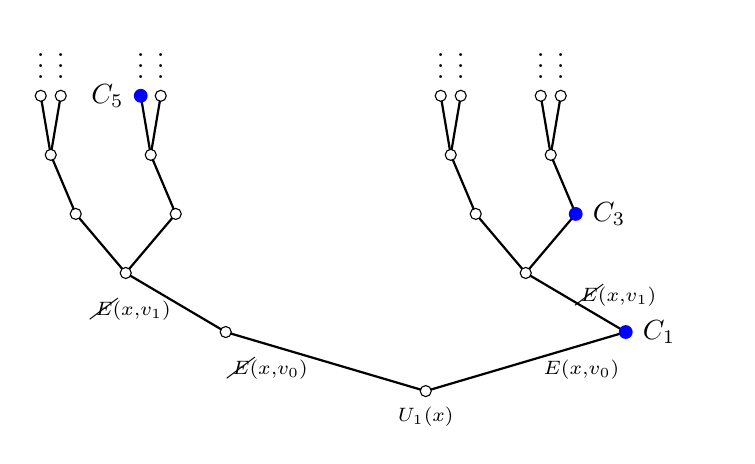
\begin{tikzpicture}[grow'=up,scale=.5]
\tikzstyle{level 1}=[sibling distance=4in]
\tikzstyle{level 2}=[sibling distance=2in]
\tikzstyle{level 3}=[sibling distance=1in]
\tikzstyle{level 4}=[sibling distance=0.5in]
\tikzstyle{level 5}=[sibling distance=0.2in]
\tikzstyle{level 6}=[sibling distance=0.1in]
\tikzstyle{level 7}=[sibling distance=0.07in]

\node {} coordinate (u9)
child{ coordinate (u0) edge from parent[color=black,thick]
child{coordinate (u00) edge from parent[color=black,thick]
child{coordinate (u000) edge from parent[color=black,thick]
child{coordinate (u0000) edge from parent[color=black,thick]
child{coordinate (u00000) edge from parent[color=black,thick]}
child{coordinate (u00001) edge from parent[color=black,thick]}
}%endparen for u0000
child{coordinate (u0001) edge from parent[color=white,thick]}
}%endparen for u000
child{coordinate (u001) edge from parent[color=black,thick]
child{coordinate (u0010) edge from parent[color=black,thick]
child{coordinate (u00100) edge from parent[color=black,thick]}
child{coordinate (u00101) edge from parent[color=black,thick]}
}%endparen for u0010
child{coordinate (u0011) edge from parent[color=white,thick]}
}%endparen for u001
}%endparen for u00
child{coordinate (u01) edge from parent[color=white,thick]}
}%endparen for u0
child{coordinate (u1) edge from parent[color=black,thick]
child{coordinate (u10) edge from parent[color=black,thick]
child{coordinate (u100) edge from parent[color=black,thick]
child{coordinate (u1000) edge from parent[color=black,thick]
child{coordinate (u10000) edge from parent[color=black,thick]}
child{coordinate (u10001) edge from parent[color=black,thick]}
}%endparen for u1000
child{coordinate (u1001) edge from parent[color=white,thick]}
}%endparen for u100
child{coordinate (u101) edge from parent[color=black,thick]
child{coordinate (u1010) edge from parent[color=black,thick]
child{coordinate (u10100) edge from parent[color=black,thick]}
child{coordinate (u10101) edge from parent[color=black,thick]}
}%endparen for u1010
child{coordinate (u1011) edge from parent[color=white,thick]}
}%endparen for u101
}%endparen for u10
child{coordinate (u11) edge from parent[color=white,thick]}
}%endparen for u1
;

%Colored nodes for right tree
\node[label=0:$C_1$,circle, fill=blue,inner sep=0pt, minimum size=5pt] at (u1) {};
\node[label=0:$C_3$,circle, fill=blue,inner sep=0pt, minimum size=5pt] at (u101) {};
\node[label=180:$C_5$,circle, fill=blue,inner sep=0pt, minimum size=5pt] at (u00100) {};

%dots going up for right tree
\node[circle,inner sep=0pt, minimum size=5pt,label=90:$\vdots$] at (u00000) {};
\node[circle,inner sep=0pt, minimum size=5pt,label=90:$\vdots$] at (u00001) {};
\node[circle,inner sep=0pt, minimum size=5pt,label=90:$\vdots$] at (u00100) {};
\node[circle,inner sep=0pt, minimum size=5pt,label=90:$\vdots$] at (u00101) {};
\node[circle,inner sep=0pt, minimum size=5pt,label=90:$\vdots$] at (u10000) {};
\node[circle,inner sep=0pt, minimum size=5pt,label=90:$\vdots$] at (u10001) {};
\node[circle,inner sep=0pt, minimum size=5pt,label=90:$\vdots$] at (u10100) {};
\node[circle,inner sep=0pt, minimum size=5pt,label=90:$\vdots$] at (u10101) {};

%empty bubble nodes
\node[label=270:$\scriptstyle{U_1(x)}$,label=20:$\hspace{1.3cm}\scriptstyle{E(x,v_0)}$,label=160:$\scriptstyle{\cancel{E}(x,v_0)}\hspace{1.3cm}$,circle, fill=white,draw,inner sep=0pt, minimum size=4pt] at (u9) {};
\node[label=160:$\scriptstyle{\cancel{E}(x,v_1)}\hspace{0.5cm}$,circle, fill=white,draw,inner sep=0pt, minimum size=4pt] at (u0) {};
\node[circle, fill=white,draw,inner sep=0pt, minimum size=4pt] at (u00) {};
\node[circle, fill=white,draw,inner sep=0pt, minimum size=4pt] at (u000) {};
\node[circle, fill=white,draw,inner sep=0pt, minimum size=4pt] at (u001) {};
\node[circle, fill=white,draw,inner sep=0pt, minimum size=4pt] at (u0000) {};
\node[circle, fill=white,draw,inner sep=0pt, minimum size=4pt] at (u00000) {};
\node[circle, fill=white,draw,inner sep=0pt, minimum size=4pt] at (u0010) {};
\node[circle, fill=white,draw,inner sep=0pt, minimum size=4pt] at (u00001) {};
\node[circle, fill=white,draw,inner sep=0pt, minimum size=4pt] at (u00101) {};
\node[label=-20:$\hspace{5mm}\scriptstyle{\cancel{E}(x,v_1)}$,circle, fill=white,draw,inner sep=0pt, minimum size=4pt] at (u10) {};
\node[circle, fill=white,draw,inner sep=0pt, minimum size=4pt] at (u100) {};
\node[circle, fill=white,draw,inner sep=0pt, minimum size=4pt] at (u1000) {};
\node[circle, fill=white,draw,inner sep=0pt, minimum size=4pt] at (u10000) {};
\node[circle, fill=white,draw,inner sep=0pt, minimum size=4pt] at (u10001) {};
\node[circle, fill=white,draw,inner sep=0pt, minimum size=4pt] at (u1010) {};
\node[circle, fill=white,draw,inner sep=0pt, minimum size=4pt] at (u10100) {};
\node[circle, fill=white,draw,inner sep=0pt, minimum size=4pt] at (u10101) {};
\end{tikzpicture}
\end{minipage}
\end{center}



\end{document}